%Version 3.1 December 2024
% See section 11 of the User Manual for version history
%
%%%%%%%%%%%%%%%%%%%%%%%%%%%%%%%%%%%%%%%%%%%%%%%%%%%%%%%%%%%%%%%%%%%%%%
%%                                                                 %%
%% Please do not use \input{...} to include other tex files.       %%
%% Submit your LaTeX manuscript as one .tex document.              %%
%%                                                                 %%
%% All additional figures and files should be attached             %%
%% separately and not embedded in the \TeX\ document itself.       %%
%%                                                                 %%
%%%%%%%%%%%%%%%%%%%%%%%%%%%%%%%%%%%%%%%%%%%%%%%%%%%%%%%%%%%%%%%%%%%%%

%%\documentclass[referee,sn-basic]{sn-jnl}% referee option is meant for double line spacing

%%=======================================================%%
%% to print line numbers in the margin use lineno option %%
%%=======================================================%%

%%\documentclass[lineno,pdflatex,sn-basic]{sn-jnl}% Basic Springer Nature Reference Style/Chemistry Reference Style

%%=========================================================================================%%
%% the documentclass is set to pdflatex as default. You can delete it if not appropriate.  %%
%%=========================================================================================%%

%%\documentclass[sn-basic]{sn-jnl}% Basic Springer Nature Reference Style/Chemistry Reference Style

%%Note: the following reference styles support Namedate and Numbered referencing. By default the style follows the most common style. To switch between the options you can add or remove �Numbered� in the optional parenthesis. 
%%The option is available for: sn-basic.bst, sn-chicago.bst%  
 
%%\documentclass[pdflatex,sn-nature]{sn-jnl}% Style for submissions to Nature Portfolio journals
%%\documentclass[pdflatex,sn-basic]{sn-jnl}% Basic Springer Nature Reference Style/Chemistry Reference Style
\documentclass[pdflatex,sn-mathphys-num]{sn-jnl}% Math and Physical Sciences Numbered Reference Style
%%\documentclass[pdflatex,sn-mathphys-ay]{sn-jnl}% Math and Physical Sciences Author Year Reference Style
%%\documentclass[pdflatex,sn-aps]{sn-jnl}% American Physical Society (APS) Reference Style
%%\documentclass[pdflatex,sn-vancouver-num]{sn-jnl}% Vancouver Numbered Reference Style
%%\documentclass[pdflatex,sn-vancouver-ay]{sn-jnl}% Vancouver Author Year Reference Style
%%\documentclass[pdflatex,sn-apa]{sn-jnl}% APA Reference Style
%%\documentclass[pdflatex,sn-chicago]{sn-jnl}% Chicago-based Humanities Reference Style

%%%% Standard Packages
%%<additional latex packages if required can be included here>

\usepackage{graphicx}%
\usepackage{multirow}%
\usepackage{amsmath,amssymb,amsfonts}%
\usepackage{amsthm}%
\usepackage{mathrsfs}%
\usepackage[title]{appendix}%
\usepackage{xcolor}%
\usepackage{textcomp}%
\usepackage{manyfoot}%
\usepackage{booktabs}%
\usepackage{algorithm}%
\usepackage{algorithmicx}%
\usepackage{algpseudocode}%
\usepackage{listings}%
%%%%

%%%%%=============================================================================%%%%
%%%%  Remarks: This template is provided to aid authors with the preparation
%%%%  of original research articles intended for submission to journals published 
%%%%  by Springer Nature. The guidance has been prepared in partnership with 
%%%%  production teams to conform to Springer Nature technical requirements. 
%%%%  Editorial and presentation requirements differ among journal portfolios and 
%%%%  research disciplines. You may find sections in this template are irrelevant 
%%%%  to your work and are empowered to omit any such section if allowed by the 
%%%%  journal you intend to submit to. The submission guidelines and policies 
%%%%  of the journal take precedence. A detailed User Manual is available in the 
%%%%  template package for technical guidance.
%%%%%=============================================================================%%%%

%% as per the requirement new theorem styles can be included as shown below
\theoremstyle{thmstyleone}%
\newtheorem{theorem}{Theorem}%  meant for continuous numbers
%%\newtheorem{theorem}{Theorem}[section]% meant for sectionwise numbers
%% optional argument [theorem] produces theorem numbering sequence instead of independent numbers for Proposition
\newtheorem{proposition}[theorem]{Proposition}% 
%%\newtheorem{proposition}{Proposition}% to get separate numbers for theorem and proposition etc.

\theoremstyle{thmstyletwo}%
\newtheorem{example}{Example}%
\newtheorem{remark}{Remark}%

\theoremstyle{thmstylethree}%
\newtheorem{definition}{Definition}%

\raggedbottom
%%\unnumbered% uncomment this for unnumbered level heads

\begin{document}

\title[Thematic Alignment in EMNLP]{Analyzing Thematic Alignment in EMNLP Conference Papers Using Sentence Embeddings}

%%=============================================================%%
%% GivenName	-> \fnm{Joergen W.}
%% Particle	-> \spfx{van der} -> surname prefix
%% FamilyName	-> \sur{Ploeg}
%% Suffix	-> \sfx{IV}
%% \author*[1,2]{\fnm{Joergen W.} \spfx{van der} \sur{Ploeg} 
%%  \sfx{IV}}\email{iauthor@gmail.com}
%%=============================================================%%

\author{\fnm{Ludovico Maria} \sur{Passoni}}\email{ludovicomaria.passoni@studenti.unimi.it}

\affil{\orgdiv{Computer science}, \orgname{Unimi}, \orgaddress{\street{Via Celoria}, \city{Milan}, \postcode{20133}, \country{Italy}}}

\abstract{This work investigates whether papers published at EMNLP 
(Empirical Methods in Natural Language Processing) are thematically 
aligned with the conference's Aims \& Scope, and whether this 
alignment has changed over the period 2019--2025. Each paper abstract 
and the Aims \& Scope text are encoded using \texttt{allenai-specter}, 
a BERT-based sentence embedding model pre-trained on scientific 
literature. An alignment score is computed for each paper as the 
cosine similarity between its embedding and the reference embedding. 
On a corpus of 330 abstracts, results show a mean alignment score of 
$0.770$ with low variability ($\sigma = 0.051$), indicating strong 
overall thematic coherence. Outlier analysis reveals that low-scoring 
papers tend to address topics at the boundary with other fields, such 
as Knowledge Graphs and computer vision, while high-scoring papers 
directly address NLP as an object of study. Temporal drift analysis 
shows substantial thematic stability across the analyzed period, with 
only a minor peak in 2023.}

\keywords{thematic alignment, NLP, EMNLP, sentence embeddings, cosine similarity}

\maketitle

\section{Introduction}\label{sec1}

This project aims to analyze thematic alignment in scientific 
conferences. Each venue publishes a document called \textit{Aims \& 
Scope}, which defines the topics the conference intends to cover. 
However, the papers that are actually published do not always fully 
reflect these stated themes. Over time, the topics addressed may drift 
away from the \textit{Aims \& Scope} and instead mirror broader 
research trends. In particular, this work analyzes the alignment 
between the \textit{Aims \& Scope} and the papers published at EMNLP 
(Empirical Methods in Natural Language Processing) over the period 
2019--2025.

To address this, I propose a methodology based on sentence embeddings 
and cosine similarity. Each paper abstract is encoded into a dense 
vector representation using \texttt{allenai-specter} \cite{specter2020}, 
a BERT-based model pre-trained on scientific literature \cite{reimers2019}. 
The same encoding is applied to the \textit{Aims \& Scope} text, which 
serves as the thematic reference. An alignment score is then computed 
for each paper as the cosine similarity between its embedding and the 
reference embedding.

The resulting scores allow me to quantify thematic coherence across 
the corpus, identify outlier papers, and detect potential thematic 
drift over time. This approach builds on recent work in bibliometric 
analysis and computational methods for understanding the evolution of 
scientific fields \cite{picascia2025, hassan2014}.

\section{Research Question and Methodology}\label{sec2}

The goal of this project is to answer the following research question: 
\textit{Are the papers published at EMNLP in the period 2019--2025 
thematically aligned with the conference's Aims \& Scope? Is there 
evidence of thematic drift over time?}

To answer this question, the following methodology was adopted:

\begin{enumerate}

\item \textbf{Data collection} --- Paper abstracts published at EMNLP 
were collected using the Semantic Scholar API, filtering only articles 
with venue ``Conference on Empirical Methods in Natural Language 
Processing''. Articles with an empty abstract were discarded, as they 
provide no useful content for the analysis. The Aims \& Scope text was 
copied from the official conference website into a plain text file and 
reformulated to provide a richer thematic reference.

\item \textbf{Content modelling} --- Both the paper abstracts and the 
Aims \& Scope text were transformed into dense numerical vector 
representations (embeddings) using \texttt{allenai-specter} 
\cite{specter2020}, a model based on Sentence-BERT \cite{reimers2019} 
and pre-trained on scientific literature.

\item \textbf{Alignment computation} --- For each abstract, an 
alignment score was computed as the cosine similarity between its 
embedding and the Aims \& Scope embedding. Cosine similarity is a 
metric used to measure how similar two vectors are, regardless of their 
magnitude, by calculating the cosine of the angle between them. It 
ranges theoretically from $-1$ to $1$, where $1$ indicates identical 
vectors and $-1$ indicates opposite vectors. In practice, embeddings 
produced by transformer-based models such as \texttt{allenai-specter} 
tend to yield positive similarity values.

\item \textbf{Results analysis} --- The alignment scores were analyzed 
statistically, visualized through a histogram, and examined over time 
to detect potential thematic drift.

\end{enumerate}

\newpage
\section{Experimental Results}\label{sec3}

\subsection{Dataset}

The corpus consists of 330 abstracts of papers published at EMNLP 
in the period 2019--2025, collected from Semantic Scholar using its 
Academic Graph API. The dataset is distributed as follows: 40 articles 
in 2019, 29 in 2020, 60 in 2021, 53 in 2022, 57 in 2023, 65 in 2024, 
and 26 in 2025.

\subsection{Metric}

The alignment score was computed as the cosine similarity between the 
embedding of the Aims \& Scope and the embedding of each abstract. 
Values range theoretically from $-1$ to $1$, however in practice, 
given the nature of transformer-based embeddings, all observed values 
fall between $0$ and $1$, where higher values indicate greater thematic 
alignment between the paper and the Aims \& Scope.

\subsection{Results}

The distribution of alignment scores is shown in Figure 
\ref{fig:histogram}. The mean score is $0.770$ with a standard 
deviation of $0.051$. The minimum score is $0.623$, corresponding 
to \textit{``A Boundary-aware Neural Model for Nested Named Entity 
Recognition''}, while the maximum is $0.918$, corresponding to 
\textit{``We are Who We Cite: Bridges of Influence Between Natural 
Language Processing and Other Academic Fields''}.

\begin{figure}[h]
    \centering
    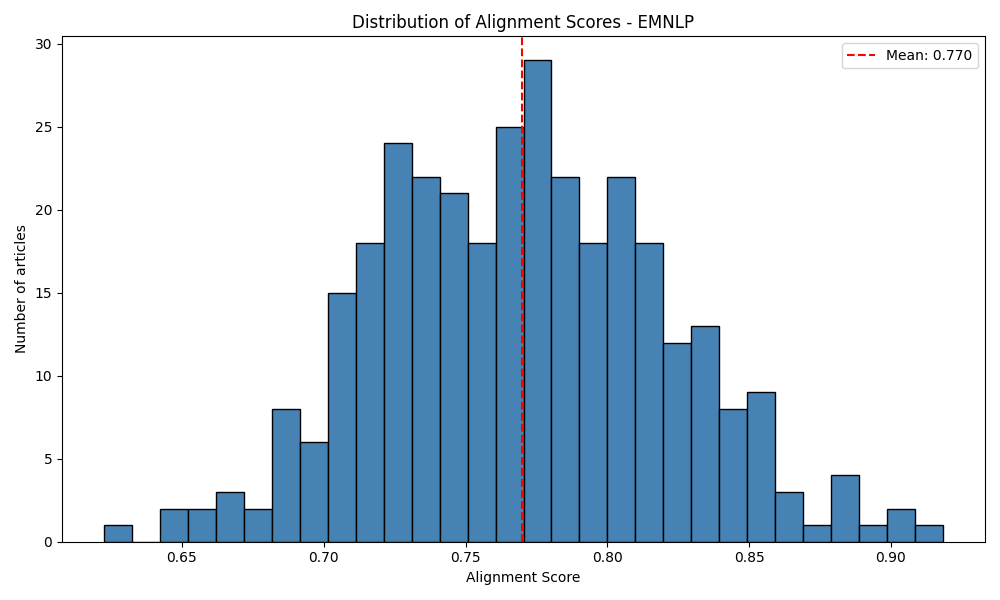
\includegraphics[width=0.8\textwidth]{histogram.png}
    \caption{Distribution of alignment scores across the EMNLP corpus (2019--2025).}
    \label{fig:histogram}
\end{figure}

The temporal drift analysis, shown in Figure \ref{fig:drift}, reveals 
a stable score around $0.757$ in the period 2019--2022, followed by 
a peak of $0.787$ in 2023, and a subsequent decline toward $0.770$ 
in 2024--2025.

\begin{figure}[h]
    \centering
    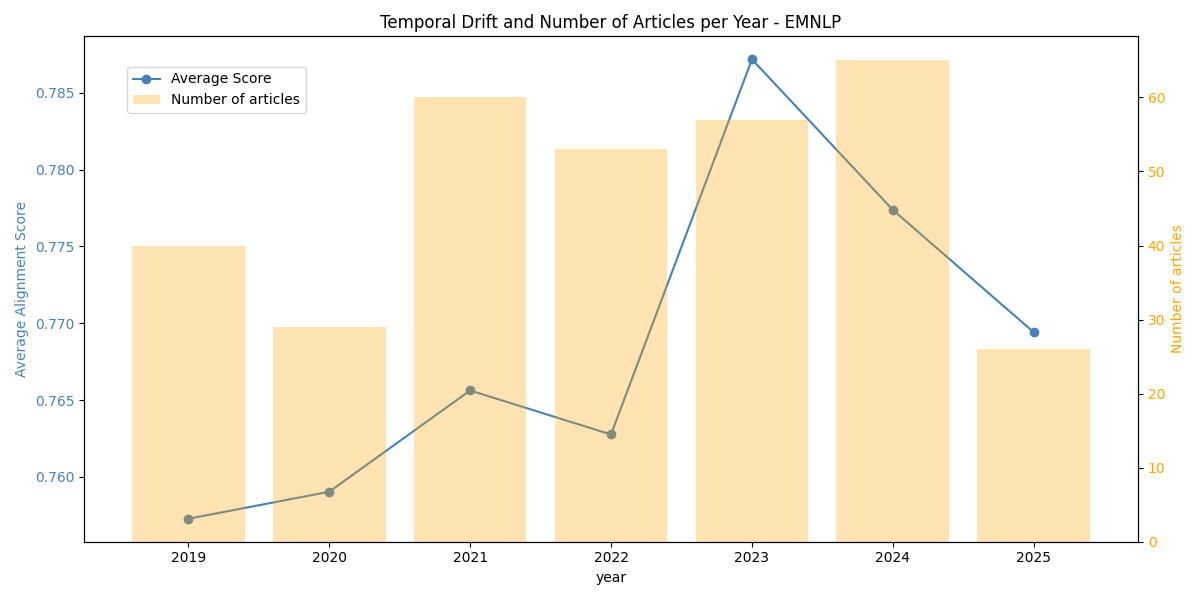
\includegraphics[width=0.8\textwidth]{drift_temporale_contestualizzato.png}
    \caption{Temporal drift of alignment scores with number of articles per year.}
    \label{fig:drift}
\end{figure}

Within the corpus, 6 low outliers (below the threshold of $0.668$, 
defined as mean $-$ $2\sigma$) and 9 high outliers (above the 
threshold of $0.872$, defined as mean $+$ $2\sigma$) were identified, 
as shown in Figure \ref{fig:outliers}. The low outliers include papers 
on Knowledge Graph embedding, multimodal retrieval, and graph neural 
networks --- topics that, while related to NLP, lie at the boundary 
with other fields such as the Semantic Web and computer vision. The 
high outliers include papers that directly address the NLP field as 
an object of study, such as bibliometric analyses, theoretical 
frameworks, and reflections on fairness and democratization in NLP 
research.

\begin{figure}[h]
    \centering
    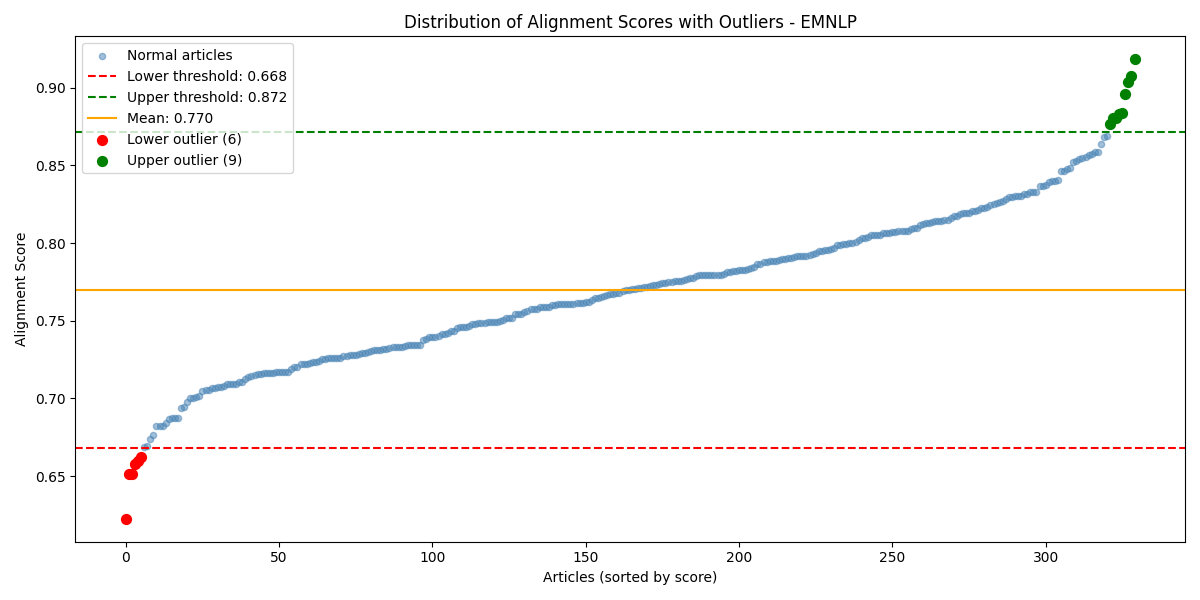
\includegraphics[width=0.8\textwidth]{outlier_plot.png}
    \caption{Distribution of alignment scores with low (red) and high (green) outliers.}
    \label{fig:outliers}
\end{figure}



\section{Concluding Remarks}\label{sec4}

The results show that the majority of papers published at EMNLP in 
the period 2019--2025 are thematically aligned with the conference's 
Aims \& Scope, with a mean alignment score of $0.770$. The relatively 
low standard deviation ($0.051$) indicates a fairly homogeneous 
distribution across the corpus.

The low outliers --- papers on Knowledge Graphs, multimodal retrieval, 
and graph neural networks --- represent works that lie at the boundary 
with other disciplines, suggesting a certain thematic openness of the 
conference toward areas adjacent to NLP. The high outliers, on the 
other hand, are papers that address NLP itself as an object of study, 
such as bibliometric analyses, theoretical frameworks, and reflections 
on fairness, and are therefore strongly aligned with the conference's 
scope.

The temporal drift observed is limited: the alignment score remains 
relatively stable throughout the analyzed period, with only a minor 
peak in 2023, suggesting that EMNLP maintains a consistent thematic 
focus over time.

\subsection{Limitations}

This study presents some limitations. First, the corpus is partial, 
as Semantic Scholar does not index all papers published at EMNLP. 
Second, the Aims \& Scope text was manually enriched with topic 
keywords from the conference's call for papers, introducing a degree 
of subjective choice into the reference representation. Finally, the 
\texttt{allenai-specter} model, while effective for scientific text, 
may not fully capture all thematic nuances present in the abstracts.

\subsection{Future Work}

Future work could explore the use of topic modelling techniques such 
as BERTopic \cite{bertopic2022} to provide a more granular thematic 
analysis. The methodology could also be extended to other NLP venues, 
such as ACL or NAACL, to enable comparative analysis across 
conferences. Finally, expanding the corpus through additional data 
sources beyond Semantic Scholar could improve the robustness of the 
results.
%%===========================================================================================%%
%% If you are submitting to one of the Nature Portfolio journals, using the eJP submission   %%
%% system, please include the references within the manuscript file itself. You may do this  %%
%% by copying the reference list from your .bbl file, paste it into the main manuscript .tex %%
%% file, and delete the associated \verb+\bibliography+ commands.                            %%
%%===========================================================================================%%

\bibliography{sn-bibliography}% common bib file
%% if required, the content of .bbl file can be included here once bbl is generated
%%\input sn-article.bbl

\end{document}
